%!TEX root = ./main.tex

\section[Why ISAC]{Why Sensing Moved Into the Network}

% SECTION TIMING: 0:00--12:00 (5 frames).
% COLOR CONVENTION FOR THE WHOLE DECK -- do not break it:
%   ranblue    = communication
%   coreorange = sensing
%   ranpurple  = adversary / illegitimate surface
%   softgreen  = the thing that survives the tradeoff
% LAYOUT RULES for this template:
%   - a frame title must fit ONE line in the title bar: keep it under ~44 characters.
%   - every bullet must fit on one line: ~30 characters in a half-width column,
%     ~25 in a 0.47 column. Shorten the text, do not let it wrap.

% Teaching note (90 s): show both photographs before saying anything. Ask what the two
% machines have in common. Students say "antennas". Push once: they also want the same
% thing -- bandwidth -- and there is only one sky.
\begin{frame}{Two machines, one sky}
  \begin{columns}[T,onlytextwidth]
    \column{0.47\textwidth}
      \centering
      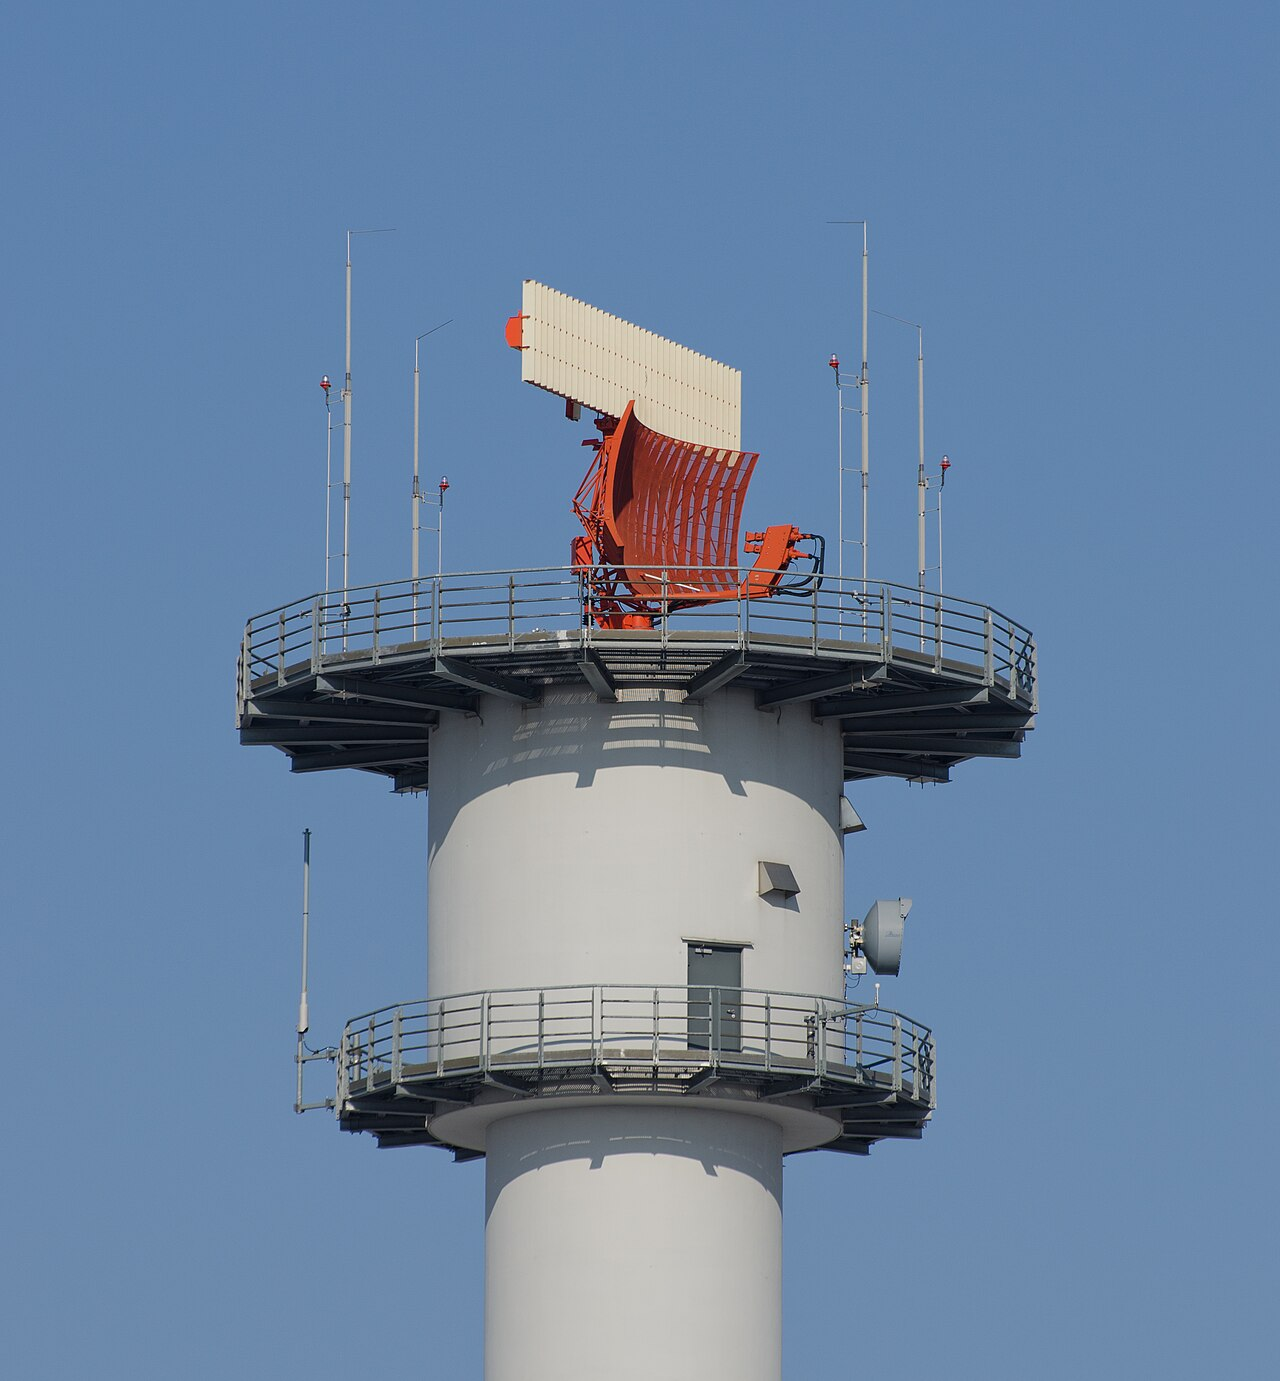
\includegraphics[height=0.42\textheight]{figure/isac/radar_surveillance.jpg}
      \source{https://commons.wikimedia.org/wiki/File:Radar_tower_airport_Frankfurt_-_Radarturm_Flughafen_Frankfurt_-_03a.jpg}{Frankfurt airport surveillance radar}
    \column{0.47\textwidth}
      \centering
      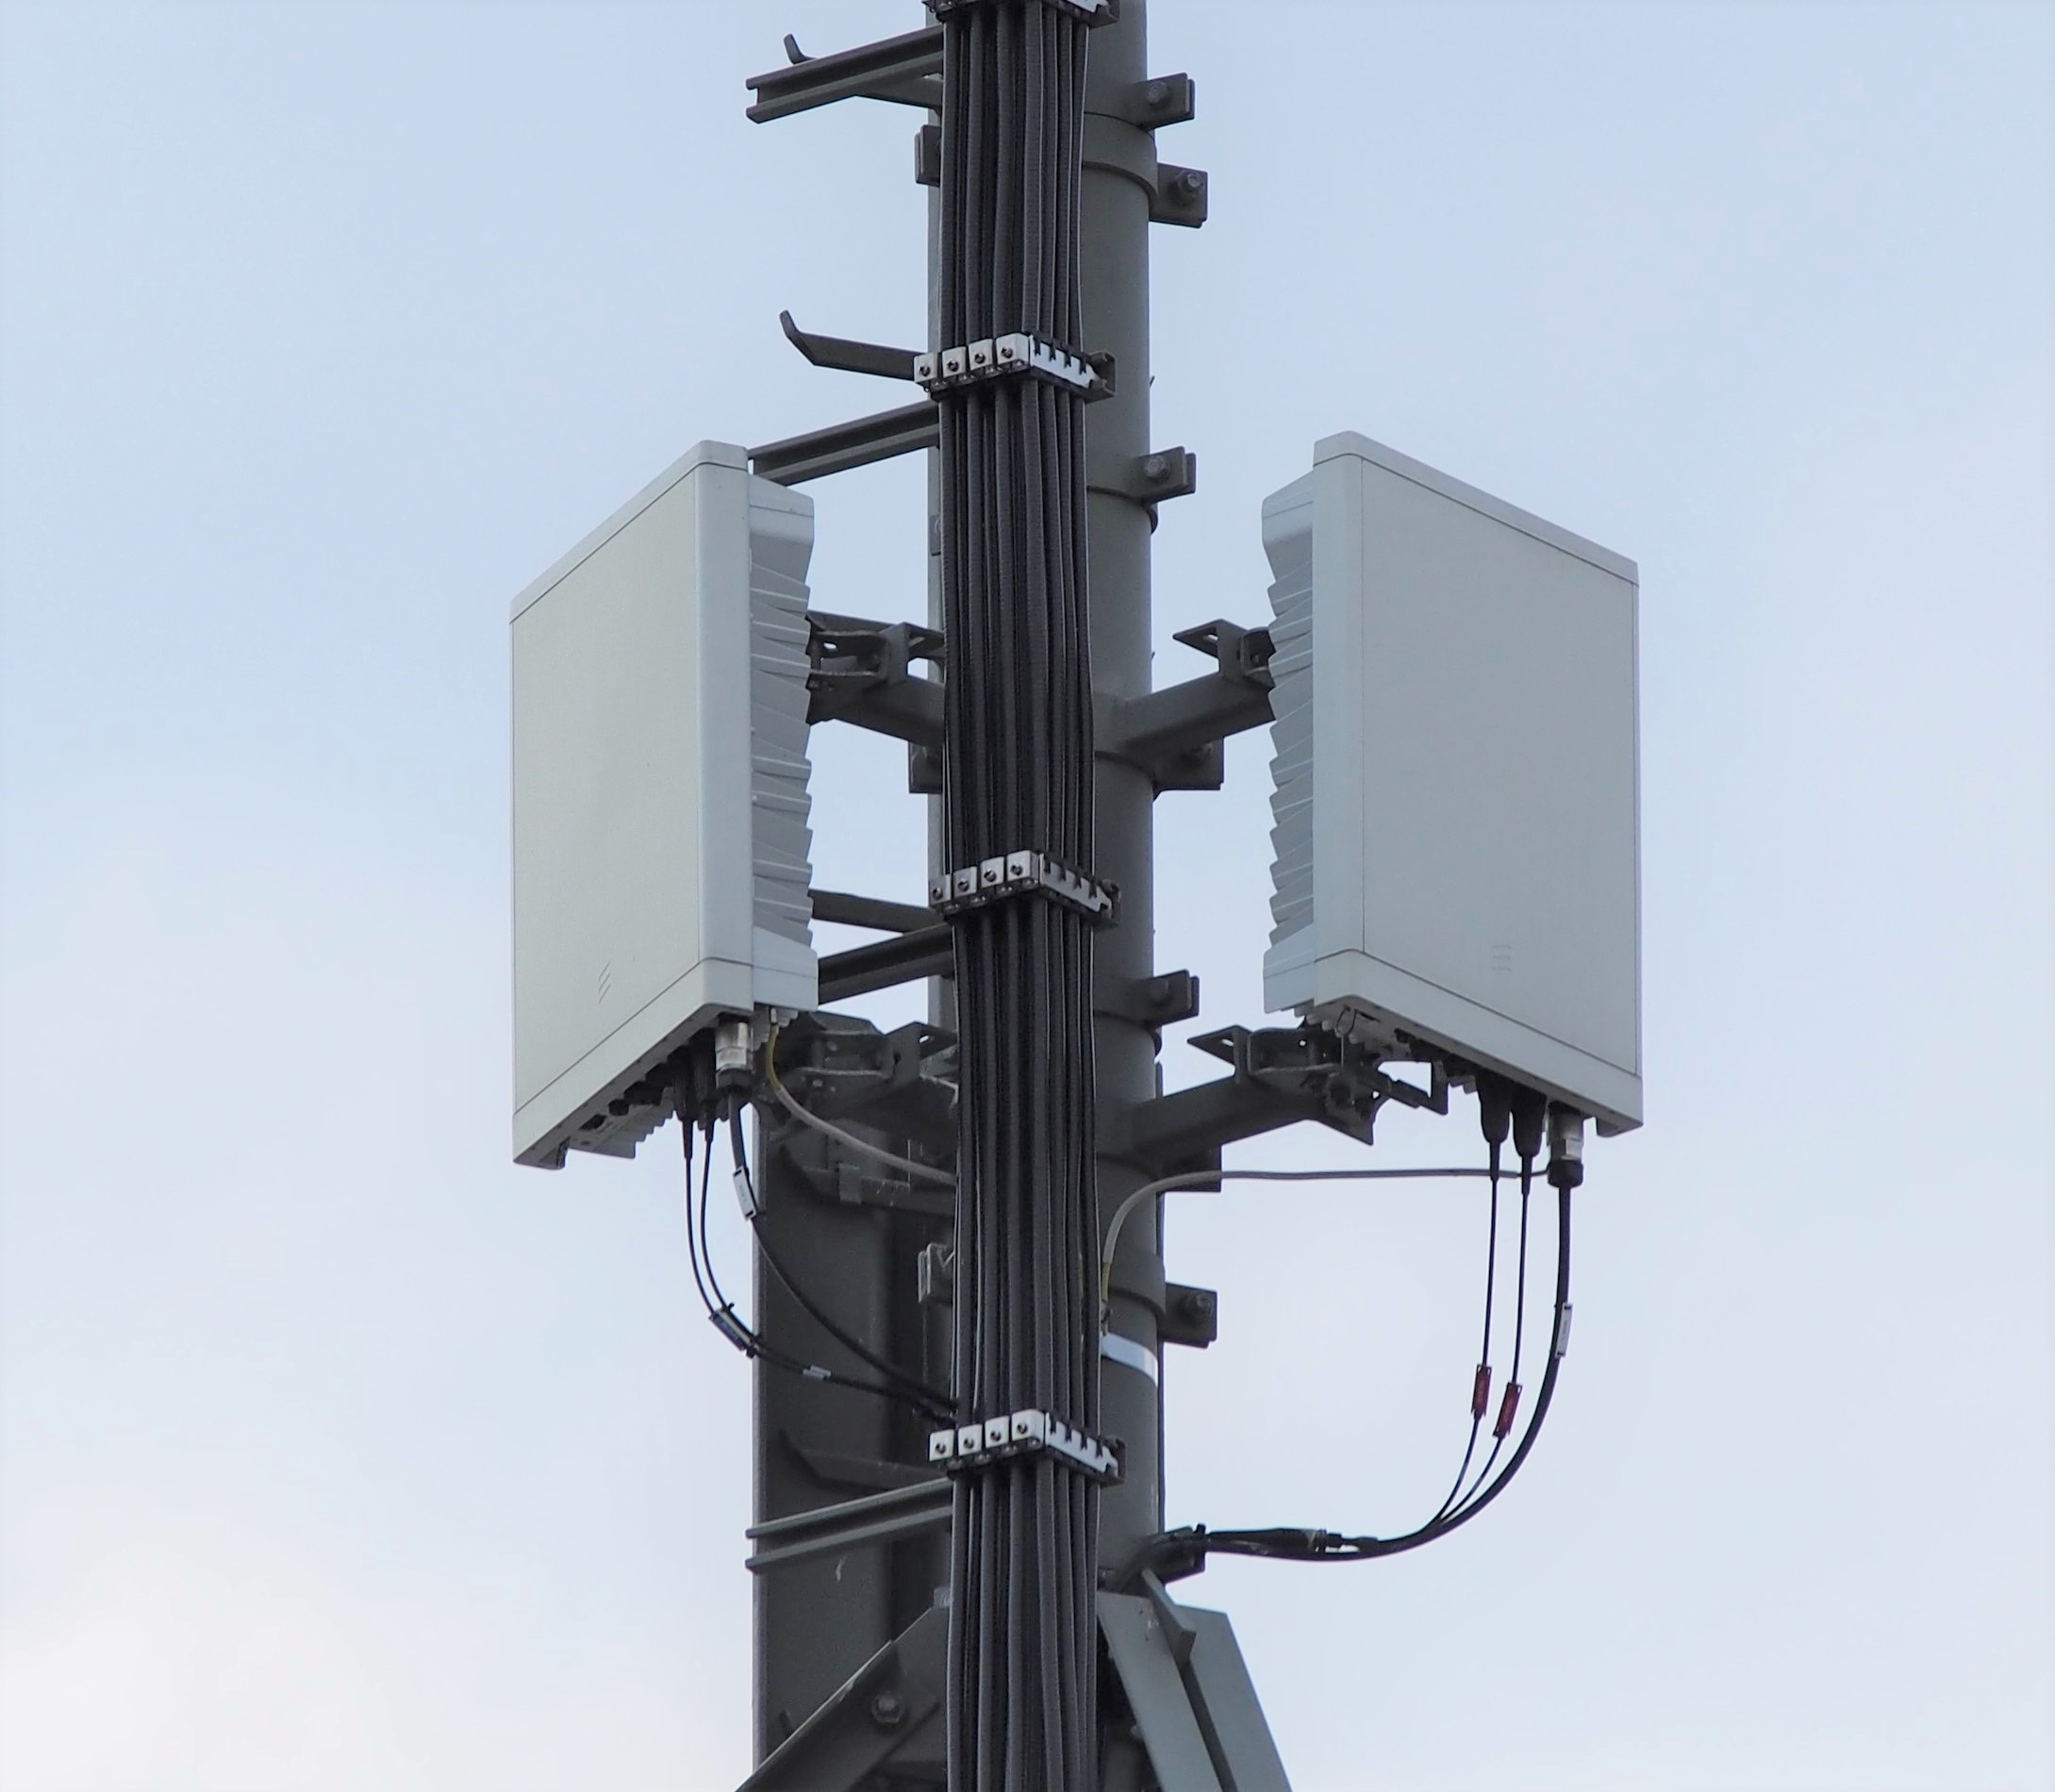
\includegraphics[height=0.42\textheight]{figure/xg/5g_antenna.jpg}
      \source{https://commons.wikimedia.org/wiki/File:Antennes_actives_5G_Ericsson.jpg}{Ericsson active 5G antennas}
  \end{columns}

  \vspace{0.4em}
  \qa{One sends a wave to be understood. One sends a wave to come back. What do they share?}
     {Spectrum, power, antennas, and silicon --- all of it scarce. Building two
      systems that never talk to each other pays for the same hardware twice.}
\end{frame}

% Teaching note (60 s): this is the one sentence of the lecture. Everything after it is
% a consequence. Do not rush past the two arrows.
\begin{frame}{One waveform, two jobs}
  \vspace{0.3em}
  \centering
  \begin{tikzpicture}[scale=0.95,transform shape]
    \node[netnode,minimum width=1.9cm] (bs) at (0,0) {ISAC BS};
    \node[netnode,minimum width=1.5cm] (ue) at (4.8,1.5) {UE};
    \node[corenode,minimum width=1.5cm] (tg) at (4.8,-1.5) {Target};
    \draw[flow,draw=ranblue,very thick] (bs)
      -- node[font=\scriptsize,text=ranblue,sloped,above,pos=0.55]{forward: carries bits} (ue);
    \draw[flow,draw=coreorange,very thick] (bs)
      -- node[font=\scriptsize,text=coreorange,sloped,above,pos=0.55]{lights up the target} (tg);
    \draw[flow,draw=coreorange,very thick,dashed] (tg)
      to[bend left=28] node[font=\scriptsize,text=coreorange,sloped,below,pos=0.5]{backward: carries an echo} (bs);
  \end{tikzpicture}

  \vspace{0.7em}
  \large
  The same transmission is \textcolor{ranblue}{information} on the way out\\[0.25em]
  and \textcolor{coreorange}{measurement} on the way back.

  \vspace{0.6em}
  \takeaway{ISAC does not add a radar to the network.\\It reads the network's own signal as radar.}
\end{frame}

% Teaching note (75 s): ask what the network could measure that an app cannot. Answers
% worth taking: presence in a room, a fall, a car two blocks away, rain.
\begin{frame}{An echo is data nobody uploaded}
  \begin{columns}[T,onlytextwidth]
    \column{0.34\textwidth}
      \centering
      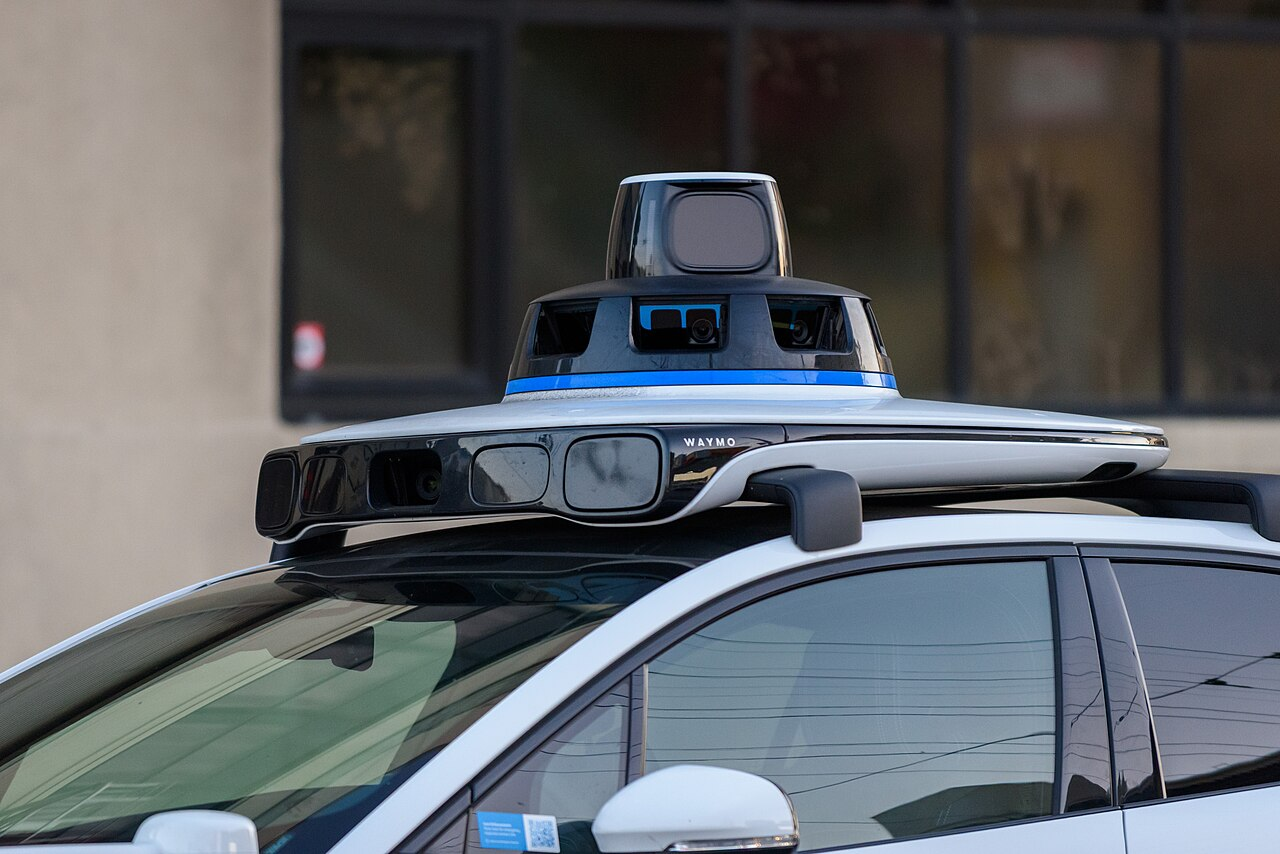
\includegraphics[width=\linewidth]{figure/isac/waymo_roof_sensor.jpg}
      \source{https://commons.wikimedia.org/wiki/File:Waymo_Jaguar_I-Pace_-_Roof_Sensor_Closeup.jpg}{Waymo Jaguar I-Pace roof sensor package}
    \column{0.62\textwidth}
      \small
      \begin{itemize}\itemsep4pt
        \item \textbf{Vehicles:} see what the camera cannot.
        \item \textbf{XR:} track a hand, no wearable.
        \item \textbf{IoT:} count people, no camera.
        \item \textbf{Space:} range the satellite you talk to.
        \item \textbf{Safety:} a drone, a fall, a flood.
        \item \textbf{Farming, weather, health:} same echo.
      \end{itemize}

      \vspace{0.5em}
      {\small\textcolor{coreorange}{\textbf{Every one of these is the network
       noticing something on its own.}}\par}
  \end{columns}

  \glossline{XR = Extended Reality \quad IoT = Internet of Things}
\end{frame}

% SOURCE: ITU-R Recommendation M.2160 (Nov 2023) defines the IMT-2030 framework and its
% six usage scenarios. ISAC is one of them. VERIFY the scenario names before class if you
% intend to list all six; only two are named here on purpose.
\begin{frame}{Sensing is written into the 6G frame}
  \vspace{0.4em}
  \centering
  \begin{tikzpicture}[scale=0.92,transform shape]
    \node[netnode,minimum width=2.5cm] (imt) at (0,0) {IMT-2030\\[-2pt]{\scriptsize the 6G framework}};
    \node[corenode,minimum width=2.4cm] (isac) at (4.6,1.05) {ISAC};
    \node[netnode,minimum width=2.4cm] (ai) at (4.6,-0.05) {AI + Communication};
    \node[netnode,minimum width=2.4cm] (etc) at (4.6,-1.15) {\ldots four more};
    \draw[flow] (imt) -- (isac);
    \draw[flow] (imt) -- (ai);
    \draw[flow] (imt) -- (etc);
  \end{tikzpicture}

  \vspace{0.9em}
  \qa{Why does a standards body have to say this out loud?}
     {Because a usage scenario is what gets spectrum, performance requirements,
      and test procedures written for it. Until ISAC was named, no radio was
      obliged to be measurable.}

  \source{https://www.itu.int/rec/R-REC-M.2160/en}{ITU-R Recommendation M.2160, IMT-2030 framework (2023)}
\end{frame}

% \begin{frame}{Where this lecture is going}
%   \vspace{0.5em}
%   \begin{columns}[T,onlytextwidth]
%     \column{0.47\textwidth}
%       \large\textbf{\textcolor{ranblue}{First half}}

%       \vspace{0.5em}
%       \small
%       \begin{itemize}\itemsep5pt
%         \item From DFRC to ISAC
%         \item OFDM, OTFS, ODDM
%         \item The tradeoff itself
%       \end{itemize}
%     \column{0.47\textwidth}
%       \large\textbf{\textcolor{coreorange}{Second half}}

%       \vspace{0.5em}
%       \small
%       \begin{itemize}\itemsep5pt
%         \item Allocation, two ways
%         \item A silent attacker
%         \item Trains, lasers, a bench
%       \end{itemize}
%   \end{columns}

%   \vspace{1.0em}
%   \ask{Keep one question open all hour:\\what does sensing cost the bits?}
% \end{frame}
